% Provenance (never printed): old seconde/premiere S material on the ocean
% (the ocean as a layered fluid, its heat, upwelling and productive waters);
% see sources/book2/PROVENANCE.md. All profiles are WOA23 columns, all
% densities the EOS-80 one-atmosphere equation, computed in
% figdata/grade-10/ocean_profiles.py.
\chapter{परतदार महासागर}\label{ch:g10:layered-ocean}

गर्मियों के किसी दिन आप तट से तैरते हुए ऐसे पानी में निकलते हैं जो सुखद रूप से गरम है।
फिर आप अपने पैर नीचे लटकाते हैं --- और आपके पैरों को सतह से कोई दो मीटर नीचे ऐसा पानी
मिलता है जो अचानक ठंडा है। समुद्र ऊपर से नीचे तक मिला हुआ नहीं है:
वह परतों से बना है, ऊपर गरम और हल्की, नीचे ठंडी और
घनी। खुले महासागर में यही परतबंदी किलोमीटरों नीचे तक पहुँचती है,
और यही तय करती है कि समुद्र कहाँ मरुस्थल है और कहाँ जीवन से भरपूर। यह
अध्याय महासागर को गहराई में देखता है: उसे कैसे मापा जाता है, उसका तापमान
और उसकी लवणता नीचे की ओर कैसे बदलते हैं, परतें स्थिर क्यों हैं, और ठंडा गहरा जल
कहाँ वापस सतह पर आता है।

\begin{recall}
समुद्री जल में लवण घुले होते हैं: उसकी लवणता, औसतन प्रति किलोग्राम समुद्री जल में लगभग
35 ग्राम लवण, एक समुद्र से दूसरे समुद्र में बदलती है। पवनें
सतही धाराओं और विशाल वृत्ताकार वलयों को चलाती हैं; ठंडे, खारे
जल की गहरी धाराएँ महासागर के तल के अनुदिश धीरे-धीरे चलती हैं (पुस्तक 1, कक्षा 8)। घनत्व द्रव्यमान को
आयतन से भाग देने पर मिलता है (भौतिकी की पुस्तकें)। पादप-प्लवक, यानी सूक्ष्म शैवाल,
को प्रकाशसंश्लेषण द्वारा बढ़ने के लिए प्रकाश और खनिज पोषक तत्त्व चाहिए, और वे
महासागर की बाक़ी खाद्य शृंखलाओं को भोजन देते हैं (जीव विज्ञान की पुस्तकें)।
\end{recall}

\section{महासागर को मापना}

महासागर लगभग \num{362}~मिलियन~\unit{km^2} पर फैला है और औसतन
\qty{3682}{m} गहरा है: लगभग \num{1.33}~अरब~\unit{km^3} जल। इसका अधिकांश भाग
प्रकाश की पहुँच से बहुत नीचे है, और इसे केवल उपकरण नीचे भेजकर ही मापा
जा सकता है।
% ledger: charette:ocean-volume

किसी जहाज़ से समुद्र-विज्ञानी एक केबल पर एक ढाँचा नीचे उतारते हैं, जिस पर लगे संवेदक
जल की चालकता (जिससे उसकी लवणता परिकलित की जाती है), उसका तापमान
और दाब (और इसलिए गहराई) मापते हैं; ढाँचे के चारों ओर बोतलों का एक घेरा होता है
जिन्हें चुनी हुई गहराइयों पर बंद किया जाता है ताकि जल के नमूने वापस जहाज़ पर लाए जा सकें।
वर्ष 2000 से रोबोटिक प्लवों के एक बेड़े ने कई मिलियन
प्रोफ़ाइल जोड़े हैं: हर प्लव \qty{1000}{m} की गहराई पर धाराओं के साथ बहता है,
लगभग हर दस दिन में \qty{2000}{m} तक डूबता है, फिर रास्ते में तापमान और लवणता
मापते हुए सतह तक उठता है, और अपना प्रोफ़ाइल
उपग्रह से भेज देता है।
% ledger: argo:fleet

\begin{dated}{2026}
अंतरराष्ट्रीय आर्गो तंत्र में लगभग 4000 सक्रिय प्लव हैं; उसका
तीस लाखवाँ प्रोफ़ाइल जुलाई 2024 में एकत्र किया गया।
% ledger: argo:fleet
\end{dated}

\begin{omfigure}
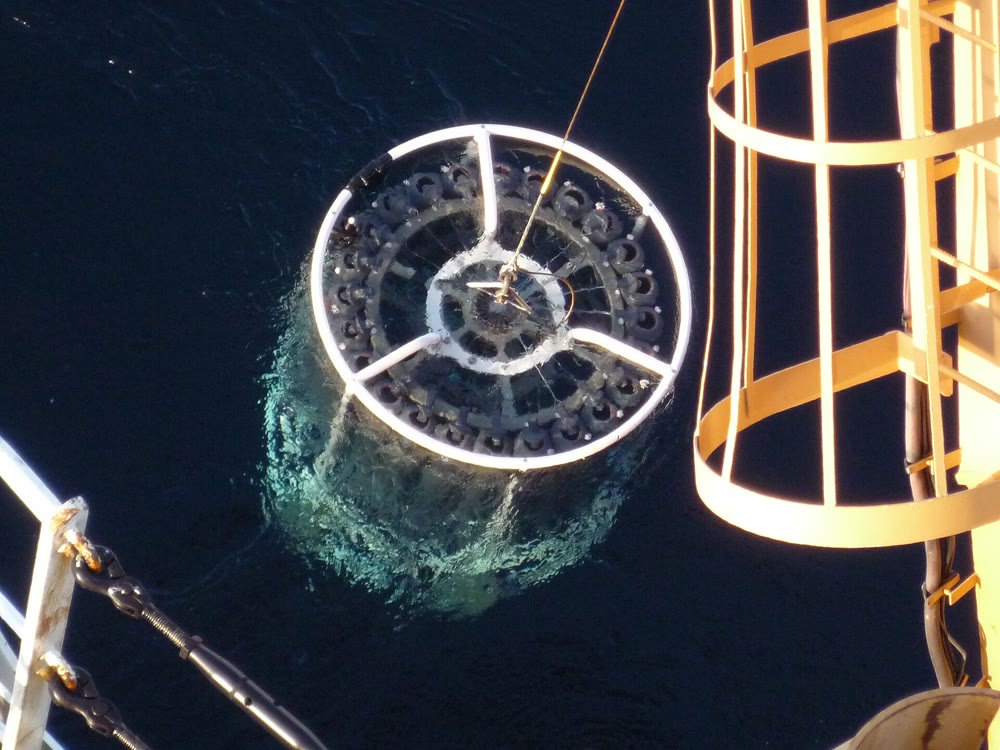
\includegraphics[height=4.4cm]{images/book2/g10-noaa-ctd-rosette.jpg}\hspace{0.4cm}%
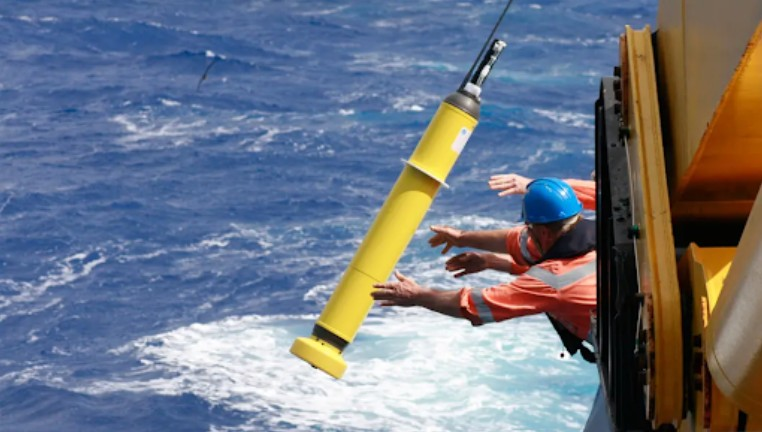
\includegraphics[height=4.4cm]{images/book2/g10-noaa-argo-float.jpg}

{\small बाएँ: अपने संवेदकों के चारों ओर नमूना-बोतलों का एक घेरा, जिसे 2008 में आर्कटिक में
एक शोध-जहाज़ के पास वापस ऊपर खींचा जा रहा है (फ़ोटो: पाब्लो
क्लेमेंते-कोलोन, NOAA फ़ोटो संग्रह)। दाएँ: एक शोध-जहाज़ से एक प्रोफ़ाइल-मापी प्लव
छोड़ा जा रहा है (फ़ोटो: NOAA का वैश्विक महासागर निगरानी एवं प्रेक्षण
कार्यक्रम)। दोनों सार्वजनिक डोमेन।}
\end{omfigure}

दशकों के मापनों पर औसत निकालने पर ये प्रोफ़ाइल महासागर का गहराई में एक
चित्र देते हैं। इस अध्याय के प्रोफ़ाइल ऐसे ही औसत हैं, जो NOAA के राष्ट्रीय पर्यावरण
सूचना केंद्र के \emph{विश्व महासागर एटलस 2023}
से लिए गए हैं।

\section{गहराई के साथ तापमान}

\begin{omfigure}
\begin{tikzpicture}
\begin{axis}[omrecord, omdepth, width=0.62\linewidth, height=8.2cm,
  axis x line=top, xmin=-3, xmax=31, ymin=0, ymax=2000,
  xlabel={तापमान (\unit{\degreeCelsius})}, ylabel={गहराई (\unit{m})},
  tick label style={font=\small}, label style={font=\small},
  legend style={font=\scriptsize, at={(0.98,0.03)}, anchor=south east}]
\addplot[omThm!85!black, thick] table[x=t, y=depth] {figdata/out/grade-10-ocean_profiles-site-warmpool.dat};
\addplot[omDef!85!black, thick] table[x=t, y=depth] {figdata/out/grade-10-ocean_profiles-site-atlantic.dat};
\addplot[black!70, thick, dashed] table[x=t, y=depth] {figdata/out/grade-10-ocean_profiles-site-arctic.dat};
\legend{{उष्णकटिबंधीय प्रशांत, 5.5\textdegree उ}, {उत्तरी अटलांटिक, 40.5\textdegree उ}, {आर्कटिक महासागर, 75.5\textdegree उ}}
\node[font=\scriptsize, anchor=west] (ml) at (axis cs:21,430) {मिश्रित परत};
\draw[black!50] (ml.north east) -- (axis cs:28.9,35);
\node[font=\scriptsize, anchor=west] (tc) at (axis cs:15.5,600) {ताप-प्रवणता परत};
\draw[black!50] (tc.north) -- (axis cs:19.9,150);
\node[font=\scriptsize, anchor=west] at (axis cs:7,1500) {गहन महासागर};
\end{axis}
\end{tikzpicture}

{\small तीन स्थलों पर गहराई के सापेक्ष औसत तापमान (गहराई नीचे की ओर
बढ़ती है)। आँकड़े: विश्व महासागर एटलस 2023, वार्षिक औसत, NOAA NCEI।}
\end{omfigure}
% ledger: data:b2-woa23 (profiles in figdata/grade-10/ocean_profiles.py)

सूर्य-प्रकाश महासागर को ऊपर से, उसकी सतही परत में, गरम करता है। पवन और लहरें इस गरम जल को
लगभग एकसमान तापमान की एक परत में मथ देती हैं। उसके नीचे तापमान कुछ
सौ मीटर में तेज़ी से गिरता है; और गहराई में वह धीरे-धीरे गिरकर उस ठंडे जल तक पहुँचता है जो
महासागरीय द्रोणियों को भरता है।

\begin{definition}[मिश्रित परत]\label{def:g10:layered-ocean:mixed-layer}
\emph{मिश्रित परत}\index{मिश्रित परत} महासागर की वह सतही परत है,
जिसे पवन और लहरें मथती हैं, और जिसमें तापमान और लवणता गहराई के साथ लगभग
नहीं बदलते।
\end{definition}

\begin{definition}[ताप-प्रवणता परत; लवण-प्रवणता परत; घनत्व-प्रवणता परत; गहन महासागर]\label{def:g10:layered-ocean:thermocline}
\emph{ताप-प्रवणता परत}\index{ताप-प्रवणता परत} \omterm{def:g10:layered-ocean:mixed-layer}{मिश्रित परत} के नीचे की वह परत है
जिसमें तापमान गहराई के साथ तेज़ी से गिरता है। जिस परत में
लवणता गहराई के साथ तेज़ी से बदलती है, वह \emph{लवण-प्रवणता परत}\index{लवण-प्रवणता परत} है;
जिस परत में घनत्व गहराई के साथ तेज़ी से बढ़ता है, वह
\emph{घनत्व-प्रवणता परत}\index{घनत्व-प्रवणता परत} है। इनके नीचे \emph{गहन
महासागर}\index{गहन महासागर} है, ठंडा और धीरे-धीरे बदलने वाला।
\end{definition}

उष्णकटिबंधीय प्रशांत में \omterm{def:g10:layered-ocean:mixed-layer}{मिश्रित परत} \qty{29.2}{\degreeCelsius} पर है और
लगभग \qty{60}{m} मोटी है; \qty{70}{m} और \qty{300}{m} के बीच तापमान
लगभग उन्नीस अंश गिरता है, और \qty{1000}{m} पर वह घटकर
\qty{4.5}{\degreeCelsius} रह जाता है। उत्तरी अटलांटिक में सतह अधिक ठंडी है और
गिरावट अधिक क्रमिक। आर्कटिक महासागर में पूरा स्तंभ \qty{0}{\degreeCelsius} के
दो अंशों के भीतर रहता है: वहाँ कहने लायक़ कोई गरम सतही परत
नहीं है।
% ledger: data:b2-woa23

\begin{method}[महासागर का प्रोफ़ाइल पढ़ना]\label{met:g10:layered-ocean:profile}
\begin{enumerate}
  \item अक्ष पहचानिए: गहराई नीचे की ओर बढ़ती है, मापी गई राशि
        ऊपर की ओर पढ़ी जाती है।
  \item \omterm{def:g10:layered-ocean:mixed-layer}{मिश्रित परत} ऊपरी भाग है जहाँ वक्र लगभग
        ऊर्ध्वाधर है; उसकी गहराई वहाँ है जहाँ वक्र मुड़ना शुरू करता है (एक प्रचलित
        नियम: जहाँ तापमान अपने सतही मान से \qty{0.5}{\degreeCelsius}
        नीचे गिर चुका हो)।
  \item \omterm{def:g10:layered-ocean:thermocline}{ताप-प्रवणता परत} वहाँ है जहाँ वक्र क्षैतिज के सबसे निकट है: सबसे
        कम गहराई में सबसे बड़ा परिवर्तन।
  \item नीचे गहरे मान पढ़िए और एक ही गहराई पर स्थलों की तुलना कीजिए।
\end{enumerate}
\end{method}

\omterm{def:g10:layered-ocean:mixed-layer}{मिश्रित परत} ऋतुओं के साथ बदलती है। सर्दियों में सतह ऊष्मा खोती है,
तूफ़ान समुद्र को मथते हैं, और \omterm{def:g10:layered-ocean:mixed-layer}{मिश्रित परत} गहरी हो जाती है; गर्मियों में सूर्य
एक पतली सतही परत को गरम करता है जिसे मंद पवनें नीचे तक मिला नहीं पातीं, और
सतह के पास एक \emph{मौसमी \omterm{def:g10:layered-ocean:thermocline}{ताप-प्रवणता परत}} बन जाती है --- वही ठंडा जल जो
तैराक के पैरों को मिलता है।

\begin{omfigure}
\begin{tikzpicture}
\begin{axis}[omrecord, omdepth, width=0.6\linewidth, height=6.6cm,
  axis x line=top, xmin=12, xmax=24, ymin=0, ymax=300,
  xlabel={तापमान (\unit{\degreeCelsius})}, ylabel={गहराई (\unit{m})},
  tick label style={font=\small}, label style={font=\small},
  legend style={font=\scriptsize, at={(0.98,0.03)}, anchor=south east}]
\addplot[omDef!85!black, thick] table[x=t_feb, y=depth] {figdata/out/grade-10-ocean_profiles-season.dat};
\addplot[omThm!85!black, thick] table[x=t_aug, y=depth] {figdata/out/grade-10-ocean_profiles-season.dat};
\legend{फ़रवरी, अगस्त}
\end{axis}
\end{tikzpicture}

{\small उत्तरी अटलांटिक में सर्दी और गर्मी (40.5\textdegree{} उत्तर,
30.5\textdegree{} पश्चिम): फ़रवरी और अगस्त के मासिक औसत तापमान।
फ़रवरी में \omterm{def:g10:layered-ocean:mixed-layer}{मिश्रित परत} लगभग \qty{170}{m} तक पहुँचती है; अगस्त में लगभग \qty{15}{m} मोटी
एक गरम परत एक मौसमी \omterm{def:g10:layered-ocean:thermocline}{ताप-प्रवणता परत} पर टिकी होती है। आँकड़े: विश्व
महासागर एटलस 2023, NOAA NCEI।}
\end{omfigure}
% ledger: data:b2-woa23 (mixed-layer depths by the 0.5 degC rule, computed in figdata/grade-10/ocean_profiles.py)

\section{लवणता और घनत्व}

समुद्री जल का घनत्व उसके तापमान और उसकी लवणता पर निर्भर करता है। इसे
अंतरराष्ट्रीय स्तर पर स्वीकृत एक सूत्र से परिकलित किया जाता है, समुद्री जल का अवस्था
समीकरण, जिसे प्रयोगशाला-मापनों पर समंजित किया गया है।

\begin{proposition}[समुद्री जल का घनत्व]\label{prop:g10:layered-ocean:density}
समुद्री जल का घनत्व उसकी लवणता के साथ बढ़ता है और उसका
तापमान बढ़ने पर घटता है। सतह के दाब पर, लवणता 35 वाले समुद्री जल का
घनत्व \qty{0}{\degreeCelsius} पर \qty{1028.1}{kg/m^3} और
\qty{25}{\degreeCelsius} पर \qty{1023.3}{kg/m^3} है;
\qty{4}{\degreeCelsius} पर शुद्ध जल का घनत्व \qty{1000.0}{kg/m^3} है।
\end{proposition}
% ledger: unesco:eos80 (values computed in figdata/grade-10/ocean_profiles.py)

\begin{omfigure}
\begin{tikzpicture}
\begin{axis}[omrecord, width=0.7\linewidth, height=6.2cm, xmin=-2, xmax=30,
  ymin=1016, ymax=1033, xlabel={तापमान (\unit{\degreeCelsius})},
  ylabel={घनत्व (\unit{kg/m^3})}, tick label style={font=\small},
  label style={font=\small}, yticklabel style={/pgf/number format/1000 sep={}}]
\addplot[omThm!85!black, thick] table[x=t, y=rho_s38] {figdata/out/grade-10-ocean_profiles-eos.dat};
\addplot[black!80, thick] table[x=t, y=rho_s35] {figdata/out/grade-10-ocean_profiles-eos.dat};
\addplot[omDef!85!black, thick] table[x=t, y=rho_s30] {figdata/out/grade-10-ocean_profiles-eos.dat};
\node[font=\scriptsize, anchor=south west, omThm!85!black] at (axis cs:1,1030.75) {लवणता 38};
\node[font=\scriptsize, anchor=south west] at (axis cs:1,1028.35) {लवणता 35};
\node[font=\scriptsize, anchor=south west, omDef!85!black] at (axis cs:1,1024.35) {लवणता 30};
\end{axis}
\end{tikzpicture}

{\small सतह के दाब पर समुद्री जल का घनत्व, उसके
तापमान के सापेक्ष, तीन लवणताओं के लिए (समुद्री जल के अंतरराष्ट्रीय अवस्था
समीकरण से परिकलित)।}
\end{omfigure}
% ledger: unesco:eos80

आरेख पर दो बातें दिखती हैं। लवणता की एक इकाई लगभग
\qty{0.8}{kg/m^3} जोड़ती है। एक अंश की तापवृद्धि \qty{25}{\degreeCelsius} पर
लगभग \qty{0.31}{kg/m^3}, \qty{10}{\degreeCelsius} पर \qty{0.18}{kg/m^3},
पर \qty{0}{\degreeCelsius} के पास केवल \qty{0.06}{kg/m^3} घटाती है: गरम समुद्रों में
घनत्व को तापमान नियंत्रित करता है, ठंडे समुद्रों में लवणता।
% ledger: unesco:eos80 (slopes computed in figdata/grade-10/ocean_profiles.py)

\begin{remark}
इस अध्याय के घनत्व सतह के दाब पर परिकलित किए गए हैं।
ऊपर के जल का दाब समुद्री जल को थोड़ा संपीडित करता है, गहराई के प्रति किलोमीटर लगभग
\qty{4}{kg/m^3}; समुद्र-विज्ञानी जल राशियों की तुलना
एक ही दाब पर करते हैं, ताकि केवल तापमान और लवणता का प्रभाव गिना जाए।
\end{remark}
% ledger: unesco:eos80-checks (computed in figdata/grade-10/ocean_profiles.py: 3.9 kg/m3 per km from the 10000-dbar check values)

\begin{omfigure}
\begin{tikzpicture}
\begin{axis}[name=sal, omrecord, omdepth, width=0.5\linewidth, height=7.2cm,
  axis x line=top, xmin=27.5, xmax=37, ymin=0, ymax=1000,
  xlabel={लवणता}, ylabel={गहराई (\unit{m})},
  tick label style={font=\small}, label style={font=\small}]
\addplot[omThm!85!black, thick] table[x=s, y=depth] {figdata/out/grade-10-ocean_profiles-site-warmpool.dat};
\addplot[omDef!85!black, thick] table[x=s, y=depth] {figdata/out/grade-10-ocean_profiles-site-atlantic.dat};
\addplot[black!70, thick, dashed] table[x=s, y=depth] {figdata/out/grade-10-ocean_profiles-site-arctic.dat};
\node[font=\scriptsize, anchor=west, align=left] at (axis cs:28.2,120) {आर्कटिक की\\लवण-प्रवणता\\परत};
\end{axis}
\begin{axis}[at={(sal.east)}, anchor=west, xshift=0.9cm, omrecord, omdepth,
  width=0.5\linewidth, height=7.2cm, axis x line=top, xmin=1021, xmax=1028.5, yticklabels={},
  ymin=0, ymax=1000, xlabel={घनत्व (\unit{kg/m^3})},
  tick label style={font=\small}, label style={font=\small},
  xticklabel style={/pgf/number format/1000 sep={}},
  legend style={font=\scriptsize, at={(0.03,0.03)}, anchor=south west}]
\addplot[omThm!85!black, thick] table[x=rho, y=depth] {figdata/out/grade-10-ocean_profiles-site-warmpool.dat};
\addplot[omDef!85!black, thick] table[x=rho, y=depth] {figdata/out/grade-10-ocean_profiles-site-atlantic.dat};
\addplot[black!70, thick, dashed] table[x=rho, y=depth] {figdata/out/grade-10-ocean_profiles-site-arctic.dat};
\legend{उष्णकटिबंधीय प्रशांत, उत्तरी अटलांटिक, आर्कटिक महासागर}
\end{axis}
\end{tikzpicture}

{\small तापमान-प्रोफ़ाइलों वाले तीन स्थलों पर गहराई के सापेक्ष लवणता (बाएँ) और सतह के दाब पर
घनत्व (दाएँ)। हर स्थल पर
घनत्व नीचे की ओर बढ़ता है। आँकड़े: विश्व महासागर एटलस 2023, NOAA NCEI;
घनत्व समुद्री जल के अंतरराष्ट्रीय अवस्था समीकरण से।}
\end{omfigure}
% ledger: data:b2-woa23, unesco:eos80

उष्णकटिबंधीय प्रशांत में \omterm{def:g10:layered-ocean:thermocline}{घनत्व-प्रवणता परत} \omterm{def:g10:layered-ocean:thermocline}{ताप-प्रवणता परत} से मेल खाती है।
आर्कटिक महासागर में तापमान लगभग नहीं बदलता, पर लवणता सतह पर 28 से,
जहाँ नदियाँ और पिघलती बर्फ़ उसे मीठा कर देती हैं, बढ़कर
\qty{500}{m} पर 34.8 हो जाती है: वहाँ \omterm{def:g10:layered-ocean:thermocline}{लवण-प्रवणता परत} ही \omterm{def:g10:layered-ocean:thermocline}{घनत्व-प्रवणता परत} है। हर स्थिति में घनत्व
नीचे की ओर बढ़ता है।
% ledger: data:b2-woa23

\begin{definition}[स्तरीकरण]\label{def:g10:layered-ocean:stratification}
महासागर \emph{स्तरित}\index{स्तरीकरण} होता है जब उसका घनत्व
गहराई के साथ बढ़ता है: हल्का जल घने जल के ऊपर परतों में टिका होता है।
\end{definition}

\omterm{def:g10:layered-ocean:stratification}{स्तरित} महासागर स्थिर होता है। घने जल में नीचे धकेला गया जल का एक पार्सल
अपने परिवेश से हल्का होता है और तैरकर वापस ऊपर आ जाता है; ऊपर धकेला गया पार्सल वापस
डूब जाता है। परतों को मिलाने के लिए पवन को इसके विरुद्ध कार्य करना पड़ता है, और
\omterm{def:g10:layered-ocean:thermocline}{घनत्व-प्रवणता परत} जितनी प्रबल हो, यह उतना ही कठिन है: \omterm{def:g10:layered-ocean:thermocline}{ताप-प्रवणता परत} एक ढक्कन है जो
सतह को \omterm{def:g10:layered-ocean:thermocline}{गहन महासागर} से अलग करता है। \omterm{def:g10:layered-ocean:thermocline}{गहन महासागर} उस जल से भरा है जो
बहुत पहले ठंडे ध्रुवीय समुद्रों से डूबा था, जहाँ सतही जल इतना घना हो जाता है कि
डूब जाए (पुस्तक 1, कक्षा 8)।

\section{उत्स्रवण}

\begin{definition}[उत्स्रवण]\label{def:g10:layered-ocean:upwelling}
\emph{उत्स्रवण}\index{उत्स्रवण} सतही परत के नीचे से ठंडे जल का ऊपर उठना है,
जो उस सतही जल का स्थान लेता है जिसे पवन दूर धकेल देती है। यह
कुछ तटों के अनुदिश और खुले महासागर में होता है।
\end{definition}
% ledger: noaa:upwelling

किसी तट के अनुदिश, किनारे के समांतर बहती पवन सतही जल को खींचती है;
पृथ्वी के घूर्णन के कारण जल केवल पवन के पीछे नहीं चलता बल्कि
उससे मुड़ जाता है, उत्तरी गोलार्ध में दाईं ओर और दक्षिणी गोलार्ध में
बाईं ओर (यह कैसे होता है, यह विश्वविद्यालय के खंडों का
विषय है)। पेरू के पास पवन किनारे के अनुदिश भूमध्य रेखा की ओर बहती है,
और सतही जल समुद्र की ओर धकेल दिया जाता है; उसका स्थान लेने के लिए तट के पास ठंडा जल
ऊपर उठता है। \omterm{def:g10:layered-ocean:upwelling}{उत्स्रवण} भूमध्य रेखा के अनुदिश भी होता है,
जहाँ व्यापारिक पवनें सतही जल को दोनों ओर उससे दूर धकेलती हैं।
% ledger: noaa:upwelling, kessler:peru-upwelling

\begin{omfigure}
\begin{tikzpicture}[font=\footnotesize, >={Stealth[length=2mm]}]
  % ocean and thermocline
  \fill[omDef!12] (0,-3.2) rectangle (8.2,0);
  \fill[omDef!30] (0,-3.2) -- (0,-2.0) .. controls (3,-2.0) and (5.5,-1.6) .. (7.4,-0.35) -- (8.2,0) -- (8.2,-3.2) -- cycle;
  \draw[omDef!80!black, dashed] (0,-2.0) .. controls (3,-2.0) and (5.5,-1.6) .. (7.4,-0.35);
  \node[anchor=north west, omDef!80!black] at (0.1,-2.05) {ताप-प्रवणता परत};
  \node[anchor=west, black!70] at (0.15,-0.9) {गरम सतही जल};
  \node[anchor=west, black!70] at (0.15,-2.75) {ठंडा, पोषक-समृद्ध जल};
  % land
  \fill[omExo!30, draw=black!60] (7.0,-3.2) -- (8.2,-0.1) -- (8.6,0.0) -- (9.6,1.2) -- (10.6,2.2) -- (10.6,-3.2) -- cycle;
  \node[anchor=south, align=center] at (9.9,-1.6) {स्थल};
  % surface flow and rising water
  \draw[->, thick, omThm!80!black] (7.2,-0.3) -- (3.6,-0.3);
  \node[anchor=south, omThm!80!black] at (5.4,-0.25) {सतही जल, तट से दूर};
  \foreach \x/\y in {6.1/-2.1, 6.8/-1.7} \draw[->, thick, omDef!80!black] (\x,\y) -- (\x+0.45,\y+1.15);
  \node[anchor=north, omDef!80!black, align=center] at (6.0,-2.25) {ठंडा जल\\ऊपर उठता है};
  % wind along the shore, northward: with west on the left and east on the
  % right the reader looks north, so the wind goes into the page
  \draw[black!70, thick] (2.6,1.0) circle (0.22);
  \draw[black!70, thick] (2.6,1.0) ++(45:0.22) -- ++(225:0.44) (2.6,1.0) ++(135:0.22) -- ++(315:0.44);
  \node[anchor=west, align=left] at (2.9,1.0) {किनारे के अनुदिश, भूमध्य रेखा की ओर पवन\\(उत्तर की ओर, पृष्ठ के भीतर)};
  \node[anchor=north west, black!60] at (0,-3.25) {$\leftarrow$ पश्चिम};
  \node[anchor=north east, black!60] at (10.6,-3.25) {पूर्व $\rightarrow$};
\end{tikzpicture}

{\small पेरू के पास तटीय \omterm{def:g10:layered-ocean:upwelling}{उत्स्रवण} (पश्चिम से
पूर्व की ओर व्यवस्था-चित्र अनुप्रस्थ काट, पैमाने पर नहीं): पवन किनारे के अनुदिश भूमध्य रेखा की ओर,
उत्तर की ओर, पृष्ठ के भीतर बहती है; सतही जल उसकी बाईं ओर मुड़कर समुद्र की ओर धकेल दिया जाता है;
\omterm{def:g10:layered-ocean:thermocline}{ताप-प्रवणता परत} के नीचे का ठंडा जल उसका स्थान लेने के लिए तट के पास ऊपर उठता है।}
\end{omfigure}

ऊपर उठने वाला जल केवल ठंडा नहीं होता। सूर्य-प्रकाशित सतही परत के नीचे,
मृत प्लवकों के अवशेष, जो डूबते और सड़ते हैं, वे खनिज पोषक तत्त्व छोड़ते हैं
जिनकी पादप-प्लवकों को आवश्यकता होती है। प्रकाश में वापस लाए जाने पर ये पोषक तत्त्व
\omterm{def:g10:layered-ocean:upwelling}{उत्स्रवण} क्षेत्रों को महासागर का सबसे उत्पादक जल बना देते हैं, जहाँ
सबसे समृद्ध मत्स्य-क्षेत्र होते हैं। जहाँ महासागर प्रबल रूप से \omterm{def:g10:layered-ocean:stratification}{स्तरित} है और कुछ भी
गहरे जल को ऊपर नहीं लाता, वहाँ सूर्य-प्रकाशित परत के पोषक तत्त्व समाप्त हो जाते हैं:
उपोष्ण वलयों के केंद्र महासागर के मरुस्थल हैं।
% ledger: noaa:upwelling

\begin{omfigure}
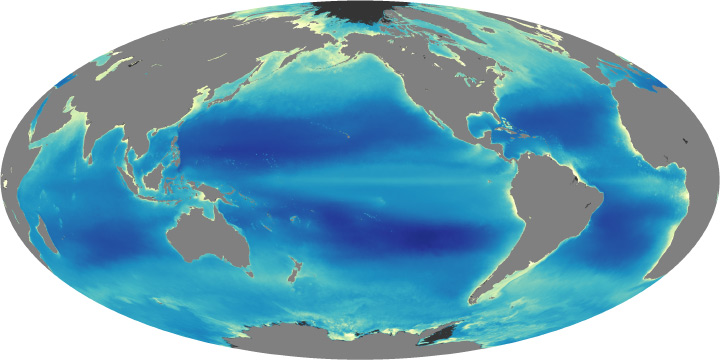
\includegraphics[width=0.8\linewidth]{images/book2/g10-nasa-ocean-chlorophyll.jpg}

{\small अंतरिक्ष से दिखता पादप-प्लवकों का पर्णहरित, 2002--2010 का औसत:
गहरे नीले (बहुत कम) से हल्के नीले होते हुए पीले (बहुत अधिक) तक;
स्थल धूसर में। पेरू का तट और प्रशांत में भूमध्य रेखा के अनुदिश की पट्टी
स्पष्ट दिखती हैं; वलय गहरे नीले हैं। चित्र: जेसी एलन और रॉबर्ट
सिमन, NASA पृथ्वी वेधशाला (सार्वजनिक डोमेन)।}
\end{omfigure}

\begin{omfigure}
\begin{tikzpicture}
\begin{axis}[omrecord, omdepth, width=0.6\linewidth, height=7.2cm,
  axis x line=top, xmin=4, xmax=26, ymin=0, ymax=600,
  xlabel={तापमान (\unit{\degreeCelsius})}, ylabel={गहराई (\unit{m})},
  tick label style={font=\small}, label style={font=\small},
  legend style={font=\scriptsize, at={(0.98,0.03)}, anchor=south east}]
\addplot[omExo!85!black, thick] table[x=t, y=depth] {figdata/out/grade-10-ocean_profiles-site-peru.dat};
\addplot[omThm!85!black, thick] table[x=t, y=depth] {figdata/out/grade-10-ocean_profiles-site-gyre.dat};
\addplot[black!40, dashed, domain=0:600, samples=2] ({15}, {x});
\legend{{पेरू के पास, 13.5\textdegree द}, {दक्षिण प्रशांत वलय, 20.5\textdegree द}}
\end{axis}
\end{tikzpicture}

{\small पेरू के पास ठंडा जल सतह के निकट आ जाता है: \qty{15}{\degreeCelsius}
का जल (डैश रेखा) लगभग \qty{65}{m} पर है, जबकि दक्षिण प्रशांत वलय के बीच में,
जो भूमध्य रेखा से अधिक दूर है, लगभग \qty{300}{m} पर। आँकड़े: विश्व महासागर एटलस 2023,
वार्षिक औसत,
NOAA NCEI।}
\end{omfigure}
% ledger: data:b2-woa23

\section{अभ्यास}

\begin{exercise}[$\star$]\label{exo:g10:layered-ocean:1}
\omterm{def:g10:layered-ocean:mixed-layer}{मिश्रित परत} और \omterm{def:g10:layered-ocean:thermocline}{ताप-प्रवणता परत} की परिभाषा दीजिए। \omterm{def:g10:layered-ocean:mixed-layer}{मिश्रित परत} को क्या मथता है?
\end{exercise}

\begin{exercise}[$\star$]\label{exo:g10:layered-ocean:2}
\omterm{def:g10:layered-ocean:upwelling}{उत्स्रवण} की परिभाषा दीजिए। \omterm{def:g10:layered-ocean:upwelling}{उत्स्रवण} क्षेत्रों का जल जीवन से समृद्ध क्यों होता है?
\end{exercise}

\begin{exercise}[$\star$]\label{exo:g10:layered-ocean:3}
तीनों स्थलों के तापमान-प्रोफ़ाइलों की सहायता से उष्णकटिबंधीय प्रशांत और आर्कटिक
महासागर में सतह पर और \qty{1000}{m} पर तापमान
बताइए।
\end{exercise}

\begin{exercise}[$\star$]\label{exo:g10:layered-ocean:4}
कौन अधिक घना है, \qty{25}{\degreeCelsius} पर लवणता 35 का समुद्री जल या
\qty{0}{\degreeCelsius} पर? एक ही तापमान पर लवणता 35 का समुद्री जल या शुद्ध जल?
अध्याय के मानों का उपयोग कीजिए।
\end{exercise}

\begin{exercise}[$\star$]\label{exo:g10:layered-ocean:5}
समझाइए कि प्रोफ़ाइल-मापी प्लव महासागर का प्रोफ़ाइल कैसे मापता है, और जहाँ जहाज़ कम ही जाते हैं वहाँ
प्लव उपयोगी क्यों हैं।
\end{exercise}

\begin{exercise}[$\star\star$]\label{exo:g10:layered-ocean:6}
महासागर \num{361.84}~मिलियन~\unit{km^2} पर फैला है और उसकी माध्य गहराई
\qty{3682}{m} है। उसका आयतन घन किलोमीटर में परिकलित कीजिए। ऊपरी \qty{100}{m} उसकी
गहराई का कितना अंश है?
\end{exercise}

\begin{exercise}[$\star\star$]\label{exo:g10:layered-ocean:7}
अगस्त के उत्तरी अटलांटिक प्रोफ़ाइल में तापमान सतह पर
\qty{22.7}{\degreeCelsius}, \qty{15}{m} पर \qty{22.2}{\degreeCelsius},
\qty{20}{m} पर \qty{21.8}{\degreeCelsius} और
\qty{50}{m} पर \qty{17.3}{\degreeCelsius} है। विधि के नियम की सहायता से
\omterm{def:g10:layered-ocean:mixed-layer}{मिश्रित परत} की गहराई का अनुमान लगाइए। \qty{20}{m} और \qty{50}{m} के बीच
तापमान गिरने की औसत दर, अंश प्रति मीटर में, क्या है?
\end{exercise}

\begin{exercise}[$\star\star$]\label{exo:g10:layered-ocean:8}
उसी उत्तरी अटलांटिक स्थल पर सतह फ़रवरी में \qty{15.3}{\degreeCelsius}
और अगस्त में \qty{22.7}{\degreeCelsius} पर है, जबकि \qty{300}{m} पर
वह दोनों महीनों में \qty{13.5}{\degreeCelsius} पर है। समझाइए कि गहरा
जल ऋतुओं का अनुसरण क्यों नहीं करता, और सर्दियों की \omterm{def:g10:layered-ocean:mixed-layer}{मिश्रित परत} गर्मियों की परत से
कहीं अधिक गहरी क्यों होती है।
\end{exercise}

\begin{exercise}[$\star\star$]\label{exo:g10:layered-ocean:9}
\qty{10}{\degreeCelsius} के पास लवणता की एक इकाई घनत्व में
\qty{0.78}{kg/m^3} जोड़ती है और एक अंश की तापवृद्धि
\qty{0.18}{kg/m^3} घटाती है। कितने अंश की तापवृद्धि लवणता की एक इकाई को
निष्प्रभावी कर देती है? यही प्रश्न \qty{0}{\degreeCelsius} के पास हल कीजिए, जहाँ एक
अंश केवल \qty{0.06}{kg/m^3} घटाता है। ध्रुवीय समुद्रों के लिए
आप क्या निष्कर्ष निकालते हैं?
\end{exercise}

\begin{exercise}[$\star\star$]\label{exo:g10:layered-ocean:10}
आर्कटिक महासागर में सतह का जल \qty{-1.4}{\degreeCelsius} पर है
और उसकी लवणता 28.1 है, और \qty{200}{m} पर जल \qty{-1.4}{\degreeCelsius} पर
है और उसकी लवणता 33.3 है। उनके घनत्व \qty{1022.6}{kg/m^3} और
\qty{1026.8}{kg/m^3} हैं। गहरे जल को क्या अधिक घना बनाता है? उनके बीच की परत का
नाम बताइए।
\end{exercise}

\begin{exercise}[$\star\star$]\label{exo:g10:layered-ocean:11}
किसी लहर द्वारा नीचे धकेले गए सतही जल के एक पार्सल की सहायता से समझाइए कि \omterm{def:g10:layered-ocean:stratification}{स्तरित} महासागर
स्थिर क्यों होता है।
\end{exercise}

\begin{exercise}[$\star\star\star$]\label{exo:g10:layered-ocean:12}
\qty{0}{\degreeCelsius} पर लवणता 35 वाले एक लीटर समुद्री जल को
\qty{25}{\degreeCelsius} तक गरम किया जाता है। अध्याय के घनत्वों की सहायता से उसका
द्रव्यमान परिकलित कीजिए, फिर उसका नया आयतन। वह कितने मिलीलीटर फैला है?
महासागर की \qty{700}{m} मोटी एक परत उसी अनुपात में गरम होती है: उसकी
मोटाई कितनी बढ़ती है? (यह महासागर के वास्तविक तापन का एक बहुत बढ़ा-चढ़ाकर लिया गया रूप है,
जिसका उपयोग यहाँ केवल प्रभाव दिखाने के लिए किया गया है।)
\end{exercise}

\begin{exercise}[$\star\star\star$]\label{exo:g10:layered-ocean:13}
उष्णकटिबंधीय प्रशांत में घनत्व \qty{50}{m} पर \qty{1021.6}{kg/m^3}
और \qty{200}{m} पर \qty{1026.0}{kg/m^3} है; फ़रवरी में उत्तरी अटलांटिक में
ऊपरी \qty{150}{m} में तापमान लगभग नहीं बदलता। दोनों में से किसमें
तूफ़ान के लिए जल को \qty{150}{m} तक मथना अधिक आसान होगा? समझाइए।
\end{exercise}

\begin{exercise}[$\star\star\star$]\label{exo:g10:layered-ocean:14}
पर्णहरित के मानचित्र पर किसी भी तट से दूर खुले महासागर में उच्च पर्णहरित के दो क्षेत्र,
और बहुत कम पर्णहरित का एक बड़ा क्षेत्र खोजिए।
अध्याय की सहायता से हर एक को समझाइए।
\end{exercise}

\begin{exercise}[$\star\star\star$]\label{exo:g10:layered-ocean:15}
मान लीजिए कि एक प्लव छह घंटों में \qty{1000}{m} से \qty{2000}{m} तक डूबता है,
फिर दस घंटों में सतह तक उठता है। हर चरण में उसकी औसत ऊर्ध्वाधर चाल
सेंटीमीटर प्रति सेकंड में परिकलित कीजिए। यदि वह उठते समय हर \qty{2}{s} पर मापन करे,
तो एक प्रोफ़ाइल में कितने मापन होते हैं, और
औसतन दो मापनों के बीच कितनी गहराई का अंतर होता है?
\end{exercise}

\section{समस्या: पेरू के पास एक मापन}

\begin{problem}[{सप्ताहांत समस्या --- दक्षिण प्रशांत के दो प्रोफ़ाइल}]
\label{pb:g10:layered-ocean:1}
% ledger: data:b2-woa23, unesco:eos80 (values rounded from figdata/grade-10/ocean_profiles.py)
तालिका दक्षिण प्रशांत के दो स्थानों पर औसत तापमान और लवणता, और
सतह के दाब पर परिकलित घनत्व देती है:
पेरू के पास (\qty{13.5}{\degree} दक्षिण, \qty{77.5}{\degree} पश्चिम) और
उपोष्ण वलय के बीच में (\qty{20.5}{\degree} दक्षिण, \qty{110.5}{\degree} पश्चिम)।

\begin{center}
\small
\begin{tabular}{c|ccc|ccc}
\hline
 & \multicolumn{3}{c|}{पेरू के पास} & \multicolumn{3}{c}{वलय} \\
गहराई (\unit{m}) & \unit{\degreeCelsius} & लवणता & \unit{kg/m^3} & \unit{\degreeCelsius} & लवणता & \unit{kg/m^3} \\
\hline
0 & 19.0 & 35.08 & 1025.08 & 24.0 & 36.41 & 1024.71 \\
25 & 17.4 & 35.06 & 1025.47 & 23.9 & 36.39 & 1024.73 \\
50 & 15.8 & 35.03 & 1025.83 & 23.6 & 36.38 & 1024.80 \\
100 & 13.7 & 34.93 & 1026.20 & 22.6 & 36.27 & 1025.02 \\
200 & 12.4 & 34.89 & 1026.44 & 20.3 & 35.80 & 1025.30 \\
300 & 11.1 & 34.80 & 1026.62 & 14.4 & 34.76 & 1025.92 \\
500 & 7.9 & 34.60 & 1026.97 & 7.1 & 34.39 & 1026.92 \\
\hline
\end{tabular}
\end{center}

\medskip
\noindent\textbf{भाग I --- प्रोफ़ाइल पढ़ना।}
\begin{enumerate}
  \item सतह पर कौन-सा स्थल अधिक गरम है, और कितना?
  \item कौन-सा स्थल भूमध्य रेखा से अधिक दूर है? क्या सतही तापमान का अंतर
        वैसा ही है जैसा आप केवल अक्षांशों से अपेक्षा करते?
  \item विधि के नियम की सहायता से वलय में \omterm{def:g10:layered-ocean:mixed-layer}{मिश्रित परत} की गहराई का
        अनुमान लगाइए।
  \item क्या पेरू के पास कोई \omterm{def:g10:layered-ocean:mixed-layer}{मिश्रित परत} है? ऊपरी \qty{100}{m} का वर्णन कीजिए।
  \item वलय में किन गहराइयों के बीच तापमान सबसे तेज़ी से गिरता है?
        दर बताइए, अंश प्रति सौ मीटर में।
  \item मोटे तौर पर, हर स्थल पर \qty{15}{\degreeCelsius} का जल किस गहराई पर
        है?
\end{enumerate}

\medskip
\noindent\textbf{भाग II --- घनत्व।}
\begin{enumerate}[resume]
  \item जाँचिए कि दोनों स्थलों पर घनत्व गहराई के साथ बढ़ता है। यह
        उनकी स्थिरता के बारे में आपको क्या बताता है?
  \item वलय में सतही जल पेरू के पास की तुलना में अधिक खारा है। इससे वह
        अधिक घना होना चाहिए या हल्का? क्या वह अधिक घना है?
  \item समझाइए कि दोनों प्रभावों में से कौन जीतता है।
  \item पेरू के पास सतह से \qty{200}{m} तक घनत्व में वृद्धि
        परिकलित कीजिए।
  \item वलय में यही वृद्धि परिकलित कीजिए।
\end{enumerate}

\medskip
\noindent\textbf{भाग III --- स्तरीकरण की तुलना।}
\begin{enumerate}[resume]
  \item वलय में ऊपरी \qty{500}{m} की घनत्व-वृद्धि का अधिकांश भाग कहाँ
        मिलता है: \qty{200}{m} के ऊपर या नीचे?
  \item पेरू के पास यह कहाँ मिलता है?
  \item \qty{500}{m} पर दोनों स्थलों की तुलना कीजिए। यह दोनों के नीचे के गहरे जल
        के बारे में क्या संकेत देता है?
  \item कुछ वाक्यों में समझाइए कि पेरू के पास \omterm{def:g10:layered-ocean:thermocline}{ताप-प्रवणता परत} को सतह की ओर
        कैसे उठा दिया गया है।
  \item पादप-प्लवक ऊपर के कुछ दसियों मीटर में रहते हैं। किस स्थल पर
        \omterm{def:g10:layered-ocean:thermocline}{ताप-प्रवणता परत} के नीचे का पोषक-समृद्ध जल पवन के मथने की
        पहुँच में है? समझाइए।
\end{enumerate}

\medskip
\noindent\textbf{भाग IV --- पेरू का जल उत्पादक क्यों है।}
\begin{enumerate}[resume]
  \item यदि किनारे के अनुदिश पवन महीनों तक बहना बंद कर दे, तो पेरू के पास सतही जल
        कैसा होगा?
  \item पर्णहरित के मानचित्र की सहायता से दोनों स्थलों की तुलना कीजिए।
  \item समझाइए कि सूर्य-प्रकाश से भरा होने के बावजूद वलय को महासागर का
        मरुस्थल क्यों कहा जाता है।
  \item पेरू के पास और वलय में सतह से \qty{200}{m} तक की घनत्व-वृद्धियों का
        अनुपात परिकलित कीजिए, और बताइए कि यह क्या दिखाता है।
\end{enumerate}
\end{problem}
